\documentclass[letterpaper,11pt]{article}
\oddsidemargin -1.0cm \textwidth 17.5cm

\usepackage[utf8]{inputenc}
\usepackage[activeacute,spanish, es-lcroman]{babel}
\decimalpoint
\usepackage{amsfonts,setspace}
\usepackage{amsmath}
\usepackage{amssymb, amsmath, amsthm}
\usepackage{comment}
\usepackage{float}
\usepackage{amssymb}
\usepackage{dsfont}
\usepackage{anysize}
\usepackage{multicol}
\usepackage{enumerate}
\usepackage{graphicx}
\usepackage[left=1.5cm,top=1.5cm,right=1.5cm, bottom=1.7cm]{geometry}
\setlength\headheight{1.5em} 
\usepackage{fancyhdr}
\usepackage{multicol}
\usepackage{hyperref}
\usepackage{wrapfig}
\usepackage{subcaption}
\usepackage{siunitx}
\usepackage{cancel}
\pagestyle{fancy}
\fancyhf{}
\renewcommand{\labelenumi}{\normalsize\bfseries P\arabic{enumi}.}
\renewcommand{\labelenumii}{\normalsize\bfseries (\alph{enumii})}
\renewcommand{\labelenumiii}{\normalsize\bfseries \roman{enumiii})}

\begin{document}

\fancyhead[L]{\itshape{Facultad de Ciencias F\'isicas y Matem\'aticas}}
\fancyhead[R]{\itshape{Universidad de Chile}}

\begin{minipage}{11.5cm}
    \begin{flushleft}
        \hspace*{-0.6cm}\textbf{FI1100 Introducción a la Física Moderna}
    \end{flushleft}
\end{minipage}

\begin{picture}(2,3)
    \put(366, -10){
\includegraphics[scale=0.9]{Imágenes/logo/dfi-fcfm.pdf}}
\end{picture}

\begin{center}
	\LARGE\textbf{Problemitas de Sonido}
\end{center}

\begin{enumerate}\setlength{\itemsep}{0.4cm}

\rfoot[]{pág. \thepage}

\begin{minipage}{0.65\linewidth}
    \item \textbf{[P3-C1 2023-1]} Un diapasón es una varilla metálica en forma de U. El sonido emitido por el diapasón contiene una sola frecuencia que viene grabada en este dispositivo y es igual a $\SI{384}{\Hz}$. El diapasón puede usarse para poder encontrar la velocidad del sonido en una columna de aire, para esto, se busca la frecuencia en la que se produce resonancia (cuando la frecuencia del diapasón coincide con algún modo normal de la columna de aire). Considere el esquema mostrado en la figura, en donde se tiene una columna de aire en un tubo de vidrio con un extremo abierto en la parte superior y cerrado en el otro lado mediante un pistón móvil. Cuando el pistón está a $\SI{22.8}{\cm}$ del extremo abierto se escucha resonando y, una vez más, cuando está a $\SI{68.3}{\cm}$ del extremo abierto.
\end{minipage}
\hfill
\begin{minipage}{0.3\linewidth}
    \begin{figure}[H]
        \centering
        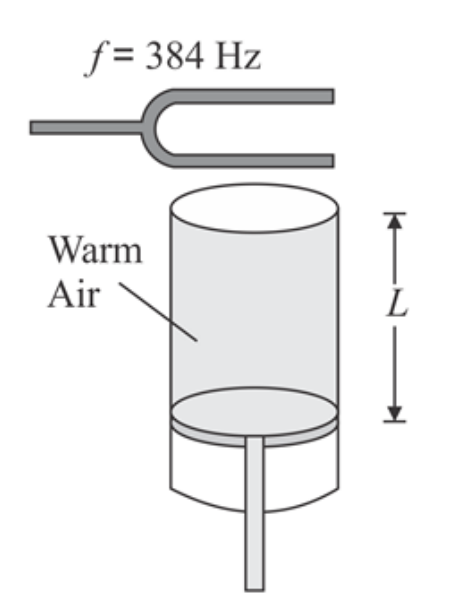
\includegraphics[width=0.9\linewidth]{Imágenes/tutorias/image.png}
    \end{figure}
\end{minipage}
\begin{enumerate}
    \item ¿Qué rapidez de sonido se implica con estos datos?
    \item ¿A qué distancia $L$ del extremo abierto estará el pistón cuando se escuche la siguiente resonancia?
\end{enumerate}

\item Al lugar de un incendio acuden por la misma carretera rectilínea, en el mismo sentido, un coche de bomberos a una velocidad $v_b$ y una ambulancia a $v_a$. Ambos coches emiten una sirena con frecuencia $f_0$. Una persona se encuentra en el costado de la carretera a una distancia $d$ del lugar del incendio escuchando las sirenas.

\begin{enumerate}
    \item En un momento dado el coche de bomberos se encuentra a una distancia $L_b$ y la ambulancia a $L_a$ del lugar del incendio, con $L_b > L_a > d$. Para la persona ubicada en la carretera, ¿cuál de los dos sonidos emitidos en ese instante llega antes?, ¿qué sirena suena más aguda?, ¿cuál es la frecuencia de la señal que oye esa persona?

    \item Para los conductores de la ambulancia y coche de bomberos, ¿cuál es la frecuencia que le llega del otro vehículo cuando se encuentran en la posición del apartado anterior?

    \item Cuando ha transcurrido un tiempo $T$, ambos vehículos hacen sonar sus sirenas otra vez. Si en esta situación se cumple que la ambulancia está a una distancia $L_a'$ y el carro de bomberos a una distancia $L_b'$ del lugar del incendio, tal que $d>L_a'> L_b'$, ¿cómo quedan los resultados de los dos apartados anteriores?
\end{enumerate}

\item Dos altavoces emiten con la misma frecuencia  y longitud de onda $\lambda=\SI{2.0}{\m}$. Estos se encuentran separados por una distancia d = 6.0m.
Una persona se encuentra a 8.0 metros frente al altavoz derecho (Considere a la persona como un punto).

a) Calcule la distancia que debe recorrer la onda generada por cada altavoz hasta la persona.

b) ¿Que tipo de interferencia sufrirán las ondas en la posición de la persona?.

c) Siguiendo el problema anterior, luego de un tiempo la persona ya se encuentra agotada del ruido (o silencio) y solo quiere estar en un lugar silencioso (o ruidoso).
Considerando que la persona se quiere mover lo menos posible y solo alejándose del altavoz derecho. ¿Cuanto debe moverse para cambiar la situación anterior?.


\end{enumerate}
\end{document}